\chapter{Foreign advisors}
\label{chap:advisors}

\section{Description of the framework}
\paragraph{}
We now proceed to definitions associated to the central matter of our thesis, which is the framework for using transformation in provelm solving with advisory information. We provide three slightly different definitions, which will later be compared in their properties. They differ in the used transformation concept. The first two frameworks use a general and widely used model of (nondeterministic) a-transducer, while the third one relies on (deterministic) sequential transducers.

\paragraph{}
\cdefinicia Let $M$ be an a-transducer and $L$ a language. Then $M_{\forall}^{-1}(L)$ is the set of all words, such that all their images belong to $L$. Formally \\
\centerline{$M_{\forall}^{-1}(L) = \{ w | M(w) \neq \emptyset \wedge M(w) \subseteq L \}$.}

\paragraph{}
\cdefinicia Let $M$ be an a-transducer and $L$ a language. Then $M_{\exists}^{-1}(L)$ is the set of words $w$, such that there is at least one image of $w$ belonging to $L$. Formally \\
\centerline{$M_{\exists}^{-1}(L) = \{ w | M(w) \cap L \neq \emptyset\}$.}


\paragraph{}
\cpriklad Let $M = (\{q_0,q_1\}, \{a\},\{b\},H,q_0,\{q_0,q_1\})$ be an a-transducer, where $H = \{(q_0,a,b,q_1),(q_1,\varepsilon,b,q_0)\}$. Moreover, let $L = \{b^2\}^*$. Every word from $a^k \in \{a\}^+$ has two images: $M(a^k) = \{b^{2k-1},b^{2k}\}$ and $M(\varepsilon) = \{\varepsilon\}$. Therefore, $M_{\forall}^{-1}(L) = \{a\}^*$,  while $M_{\exists}^{-1}(L) = \{\varepsilon\}$. 

\paragraph{}
\cdefinicia Let $L_{dec}$ be a regular language. Let $q \in \{\forall,\exists\}$. A pair $(L_{adv}, M)$, where $L_{adv}$ is a regular language and $M$ an a-transducer is called an \emph{$NT_{q}$-advice with regard to $L_{dec}$}, if there exists a deterministic finite automaton $A'$, such that $L_{dec} = L[M_{q}^{-1}(L_{adv})](A')$. Moreover, $(L_{adv}, M)$ is called \emph{effective}, if $\C{A'} + \C{M} + \C{L_{adv}} \leq	 \C{L_{dec}}$.

\paragraph{}
\cpriklad Let $L_{dec} = \{ a^{12k}| k \geq 0 \} $. Let $M= (\{q_0, q_1\}, \{a\}, \{a\}, H, q_0, \{q_0\})$, where $H = \{(q_0, a, a, q_1), (q_1, a, \varepsilon, q_0)\}$ and $L_{adv} = \{ a^{2k}| k \geq 0 \}$. $M$ shortens every word from $a^*$ to half of its length, so it is easy to see, that $M_{\forall}^{-1}(L_{adv}) = M_{\exists}^{-1}(L_{adv}) = \{ a^{4k}| k \geq 0 \}$. We now construct a simpler finite automaton $A'$ for the language $L_{simple} = \{ a^{3k}| k \geq 0 \}$. Clearly, $\C{A'} + \C{M} + \C{L_{adv}} = 3 + 2 + 2 \leq 12 = \C{L_{dec}}$ and $L[M^{-1}_{\forall}L_{adv}](A') = L[M^{-1}_{\exists}L_{adv}](A') = L_{dec}$ which means, that $L_{adv}$ with $M$ is an effective $NT_{\forall}$- and $NT_{\exists}$-advice with regard  to $L_{dec}$.

\paragraph{}
\cpriklad Let $L_{dec} = \{ a^{3k}|k \geq 0 \} \cup \{ a^{5k}|k \geq 0\}$. Now, let $M$ be an a-transducer from Figure 4.1, $L_{adv} = L_{simple} = \{a\}^*$. We can see, that $M$ has accepting computations only on words from $L_{dec}$ and so $M^{-1}_{\exists}(L_{adv}) = M^{-1}_{\forall}(L_{adv}) = L_{dec}$. $\C{M} + \C{L_{simple}} + \C{L_{adv}} = 11$, while $\C{L_{dec}} = 15$ (this could be proven by Myhill-Nerode theorem), so $(L_{adv},M)$ is an effective $NT_{\forall}$- and $NT_{\exists}$-advice with regard  to $L_{dec}$.

\begin{figure}[h!]
\centering
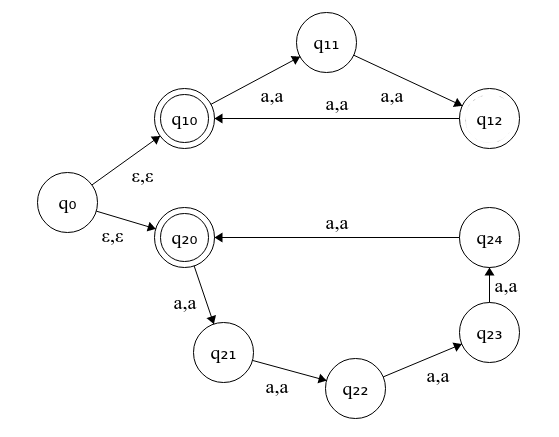
\includegraphics[scale=0.5]{mainmatter/images/nondet.png}
\caption{a-transducer $M$}
\end{figure}

\paragraph{}
In the last example, the whole advice was in some sense contained in the transformation and the efficiency was achived just through the nondeterminism of a-transducer. We would like to prevent such a misuse of the nondeterminism, so the saving of state count would mirror the actual possibility to dismember the problem to some smaller subproblems, such that their results combined yield the solution of the whole task.

\paragraph{}
At first sight on the previous example it seems, that the problem lays in the fact, that $M$ does not have to generate the whole language $L_{adv}$. The one possible solutions is to add a condition, that the filtering of words not from $L_{dec}$ should not happen only in $M$, but also in $L_{dec}$ (and since the complexity of $L_{dec}$ is the state count of its minimal deterministic automaton, the nondeterminism could not be misused). Formally, a pair $(L_{adv}, M)$ is a ($NT_{\forall}$-) $NT_{\exists}$-advice with regard  to $L_{dec}$, if it fulfills the condition from the original definitions and moreover, we demand, that $L_{adv} \subseteq M(\Sigma_{L_{dec}}^*)$.

\paragraph{}
However, if we alter the a-transducer $M$, so that each travelsal of form $(q_i,a,a,q_j)$ will be altered to $(q_i,a,\varepsilon,q_j)$, we can take $L_{dec} = \{\varepsilon\}$. Again, $M^{-1}_{\exists}(L_{adv}) = M^{-1}_{\forall}(L_{adv}) = L_{dec}$ and the complexity of the advice has increased by $1$ (since $\C{\{\epsilon\}} = 2$), so $(L_{adv},M)$ still is an effective advice for $L_{dec}$. However, our problem with the misuse of nondeterminism is still apparent. Adding this simple condition did not help at all.

\paragraph{}
For aforementioned reason, we present the third possible definition of our framework, where the transformation model is not an a-transducer, but a (deterministic) sequential transducer. However, unlike by a-transducer, one-bounded sequential transducers are not a normal form of sequential transducers. It is easy to see, that with this restriction, the we cannot generate an output word, which is longer than the input. However, this shortcoming can be easily solved by a little alternation in a definition:
\begin{itemize}
\item $\delta$ is a partial transition function, that maps $K \times \Sigma_{1} \cup \{\varepsilon\} \rightarrow K$,
\item $\sigma$ is a partial output function, that maps $K \times \Sigma_{1} \cup \{\varepsilon\} \rightarrow \Sigma_{2}$,
\item however, the $\epsilon$-transition and $\epsilon$-output in a state $q \in K$ are possible only if $q \in F$ (this transition has to be mandatory) there are no other transitions and outputs in this state, and
\item since $\delta$ and $\sigma$ are partial functions, we demand, that for $a \in \Sigma_1 \cup \{\varepsilon\}$ and $q \in K$, $\delta(q,a)$ is defined, if and only if $\sigma(q,a)$ is defined.
\end{itemize}

\paragraph{}
It can be easily shown, that this altered definition is a normal form of sequential transducers, however, we do not include the proof in our thesis.

\paragraph{}
\cdefinicia Let $M$ be a sequential transducer and $L$ a language. Then $M_{D}^{-1}(L)$ is the set of all words, such that their images belong to $L$. Formally \\
\centerline{$M_{D}^{-1}(L) = \{ w | M(w) \in L \}$.}

\paragraph{}
\cdefinicia Let $L_{dec}$ be a regular language. A pair $(L_{adv}, M)$, where $L_{adv}$ is a regular language and $M$ a sequential transducer is called an \emph{$T$-advice with regard to $L_{dec}$}, if there exists a deterministic finite automaton $A'$, such that $L_{dec} = L[M_{D}^{-1}(L_{adv})](A')$. Moreover, $(L_{adv}, M)$ is called \emph{effective}, if $\C{A'} + \C{M} + \C{L_{adv}} \leq	 \C{L_{dec}}$.

\paragraph{}
\cpriklad We can see, that the a-transducer $M$ from Example 2 has neither $\varepsilon$-transitions, nor multiple transitions from one state on one symbol. Moreover, the transition function is complete (the set $H$ contains an element for every combination of source state and input symbol), so the corresponding sequential transducer $M_D$ and its transition function $\delta$ and output function $\sigma$ can be easily constructed. Therefore, the pair $(L_{adv},M)$ from Example 2 is an effective $M_{D}$-advice with regard to $L_{dec}$.

\paragraph{}
\poznamka We will often use this view of a sequential transducer - as a special case of an a-transducer. When it will be suitable, we will identify a sequential transducer with an a-transducer, which set $H$ fulfills the aforementioned conditions (no $\varepsilon$-transitions and for each combination of state and input symbol precisely one element in $H$) without the formal definition of its $\delta$ and $\sigma$ functions. We state their construction here.

\centerline{$\forall h \in H: \delta(pr_0(h),pr_1(h)) = pr_3(h)$}
\centerline{$\forall h \in H: \sigma(pr_0(h),pr_1(h)) = pr_2(h)$}

\paragraph{}
The correctness of the definition of these function follows from the "determinism" of $H$.

\paragraph{}
We have defined three alternative ways to look at the use of transformation in solving problems with advisory information, which differ in the definition of the language $M^{-1}(L)$. This brings up the following question: for a given language $L$ and an a-transducer $M$, how to get the languages $M_{\forall}^{-1}(L)$, $M_{\exists}^{-1}(L)$ and $M_{D}^{-1}(L)$? The answer was quite easy to find in previous two examples (and, in fact, for all languages in form $\{ (a^k)^* \}$ and transducers, which just manipulate the number of symbols $a$). We now look at the answer in general.

\paragraph{}
\clema Let $M = (K, \Sigma_1, \Sigma_2, H, q_0, F)$ be an a-transducer and $L$ a language. Moreover, let $L' = M_{\exists}^{-1}(L)$. Then $\forall w \in L'^c: M(w) = \emptyset \vee M(w) \subseteq L^c$. The mapping $M_{\exists}^{-1}$ can be simulated by an a-transducer $M'$ dual to $M$, such that $M'(L) = L'$, where $\C{M'} = \C{M}$.

\paragraph{}
\dokaz The first part is quite easy to see, since by definition, $M_{\exists}^{-1}(L)$ contains all words, such that at least one of their images by a-transducer $M$ belongs to $L$. If for a word $v \in L'^c$ there is a word $u$, such that $u \in M(v)$ and $u \notin L^c$, then $u \in L$ and by definition, $v \in L'$, which leads to a contradiction.

\paragraph{}
We prove the second part of our Lemma constructively. Let $M' = (K, \Sigma_2, \Sigma_1, H', q_0, F)$, where\\
\centerline{$H'=\{(p,x,y,q)|(p,y,x,q) \in H\}$.} 

\paragraph{}
Clearly, $\C{M} = \C{M'}$. It remains to show, that $M'$ simulates $M_{\exists}^{-1}$, namely that $M'(L) = L'$ (since $L' = M_{\exists}^{-1}(L)$).
\begin{itemize}
\item $L' \subseteq M'(L)$: Take an arbitrary word $u \in L'$. By definition of $M_{\exists}^{-1}$, there is a word $v \in L$, such that $v \in M(u)$. Now, let us look at this computation of $M$ on $u$ as a word $h \in \Pi_M$ (see Chapter 1). Since this computation is accepting and its output is $v$, we can rewrite $h$ as a sequence of quadruples $(q_0, x_1, y_1, p_1)$ $(p_1,x_2,y_2,p_2)...$ $(p_{i-1},x_i,y_i,p_i)...$$(p_{n-1},x_n,y_n,q_F)$, where $pr_1(h) = u$, $pr_2(h) = v$ and $q_F \in F$. We now present the computation of $M'$, which shows, that $u \in M'(v)$. The computation is $h' \equiv (q_0, y_1, x_1, p_1)$$(p_1,y_2,x_2,p_2)...$ $(p_{i-1},y_i,x_i,p_i)...$$(p_{n-1},y_n,x_n,q_F)$. The plausibility of this computation follows from the construction of $M'$. We have shown, that $u \in M'(L)$ and therefore $L' \subseteq M'(L)$.
\item $M'(L) \subseteq L'$: Once again, let us take a word $u \in M'(L)$. There is a word $v \in L$, such that $u \in M'(v)$. Again, we can look at the respective computation of $M'$ on $v$ as a word $h' \equiv (q_0, y_1, x_1, p_1)$$(p_1,y_2,x_2,p_2)...$ $(p_{i-1},y_i,x_i,p_i)...$$(p_{n-1},y_n,x_n,q_F)$, where $pr_1(h') = v$ and $pr_2(h') = u$. We construct the computation $h$ of $M$ in the same way as in previous part of the proof. The computation $h$ shows, that $v \in M(u)$ and therefore $M(u) \subseteq L$ (whole $M(u)$, since all words $v$, such that $u \in M'(v)$ have to belong to $L$ according to the first part of Lemma). From the definition of $M_{\exists}^{-1}$ it follows, that $u \in M_{\exists}^{-1}(L) = L'$.
\end{itemize} \qed

\paragraph{}
Very similar result can be stated for the setting with a sequential transducer. For a sequential transducer $M$ and a language $L$, $M_{D}^{-1}(L) = M_{\exists}^{-1}(L)$, since every word $w \in M^{-1}_{D}(L)$ has exactly one image $M(w) \in L$. This means, that we can find $L$ using the same dual a-transducer $M'$. Note, that this dual machine does not necessarily be a sequential transducer, because the mapping by $M$ is not necessarily injective (and even if it is, the functions $\delta$ and $\sigma$ do not say anything about uniqeness of the combination of output symbol and resulting state). However, the determinism of the sequential transducer allows us to state some additional claims.

\paragraph{}
\clema Let $M = (K, \Sigma_1, \Sigma_2, \delta, \sigma, q_0, F)$ be a sequential transducer and $L$ a language. Moreover, let $L' = M_{D}^{-1}(L)$. Then, $M(L') \subseteq L$ and $\forall w \in L'^c: M(w) = \emptyset \vee M(w) \in L^c$. The mapping $M_D^{-1}$ can be simulated by an a-transducer $M'$ dual to the sequential transducer $M$, such that $M'(L) = L'$ and $\forall w \in L^c: M'(w) = \emptyset \vee M'(w) \subseteq L'^c$. Moreover, $\C{M'} = \C{M}$.

\paragraph{}
\dokaz We prove just that parts of our Lemma, which are different from the claims in the previous one. In the first part, we state, that $M(L') \subseteq L$. This claim follows directly from the fact, that every word $w \in L'$ has only one image $M(w)$ and by definition, this image belongs to $L$ (otherwise $w \notin L'$). Moreover, since the image of a word $w$ by a sequential transducer is a word, instead of a set, the condition on words from $L'^c$ changes accordingly.

\paragraph{}
We provide the formal construction of the a-transducer $M'$, since we construct it from the sequential transducer $M$. Again, $M' = (K,\Sigma_1,\Sigma_2,H,q_0,F)$, where \\
\centerline{$H = \{q,a,\sigma(a),\delta(q) | \forall q \in K, a \in \Sigma_1 \}$.}

\paragraph{}
The proof of the claim, that $M'(L) = L'$, is very similar to the proof of previous Lemma. We provide the arguments for the last part of Lemma, i. e. $\forall w \in L^c: M'(w) = \emptyset \vee M'(w) \subseteq L'^c$: Assume there is a word $w \in L^c$, such that $M'(w) = u \wedge u \in L'$. From previous part of Lemma it follows, that $u \in M'(L)$. However, then $w = M(u) \subseteq L$, which leads to a contradiction. \qed

\paragraph{}
We have seen, that finding the sets $M_{\exists}^{-1}(L)$ and $M_D^{-1}(L)$ for a given language $L$ and transducer $M$ is quite easy using a dual a-transducer $M'$. However, the situation with $M_{\forall}^{-1}$ is not that simple. The main problem is, that if some word $w \in \Sigma_{L'}^*$ has an image $L$, it can also have other images in $L^c$, therefore $w \notin L'$. However, if we used a dual a-transducer $M'$ from previous Lemmas on $L$, the word $w$ will be constructed, since $w \in M'(L)$. We now present the solution to this issue.

\paragraph{}
\clema Let $M = (K, \Sigma_1, \Sigma_2, H, q_0, F)$ be an a-transducer and $L$ a language. Moreover, let $L' = M_{\forall}^{-1}(L)$. Then, $M(L') \subseteq L$. The mapping $M_{\forall}^{-1}$ can be simulated by an a-transducer $M'$ dual to the sequential transducer $M$, such that $L' = M'(L) - M'(L^c)$ and $\forall w \in L^c: M'(w) = \emptyset \vee M'(w) \subseteq L'^c$. Moreover, $\C{M'} = \C{M}$.

\paragraph{}
\dokaz The first part ($M(L') \subseteq L$) follows from the definition. If a word $w$ belongs to $L'$, all of its images by $M$ are in $L$, therefore whole $M(w) \subseteq L$ and furthermore $M(L') \subseteq L$.

\paragraph{}
Now we prove the second claim in three steps, using the same construction of the dual a-transducer $M'$ as before.
\begin{itemize}
\item $L' \subseteq M'(L) - M'(L^c)$: Let $w \in L'$. By definition, $M(w) \neq \emptyset \wedge M(w) \subseteq L$, therefore, there is a word $u \in M(w) \wedge u \in L$. By the construction of $M'$, it can be easily seen (and proven similarly to the proof of the $M_{\exists}^{-1}$ case), that $w \in M'(u) \subseteq M'(L)$. Furthermore, if $w \in M'(L^c)$, it means, that there is a word $v \in L^c$, such that $w \in M'(v)$. However, then $v \in M(w)$ and since $v \notin L$, then $M(w) \not \subseteq L$ and by definition $w \notin L'$.

\item $M'(L) - M'(L^c) \subseteq L'$: Let $w \in M'(L) - M'(L^c)$. Since $w \in M'(L)$, we know, that there is at least one word $u$, such that $u \in L \cap M(w)$. The second part, i. e. $w \notin M'(L^c)$ secures, that $L^c \cap M(w) = \emptyset$ (if there was a word $u \in L^c \cap M(w)$, then $w \in M'(u) \subseteq M(L^c)$). Thus, $w$ fulfills the definition of $M^{-1}_{\forall}(L)$, therefore $w \in L'$.

\item $\forall w \in L^c: M'(w) = \emptyset \vee M'(w) \subseteq L'^c$: This claim follows directly from the fact, that $L' \cap M'(L^c) = \emptyset$.
\end{itemize} \qed

\paragraph{}
We conclude this section with a note, which will later be useful by comparing our three settings to each other. This its claim follows directly from the fact, that a sequential transducer is a special case of an a-transducer and the definition of $M^{-1}_{D}$ fulfills the definitions for both $M_{\forall}^{-1}$ and $M_{\exists}^{-1}$.

\paragraph{}
\poznamka Every (effective) $T$-advice is also a $NT_{\forall}$-advice. Every (effective) $T$-advice is a $NT_{\exists}$-advice.

\section{Decomposable and undecomposable languages}

\paragraph{}
In the previous section, we have defined the notion of an effective advice. Now we present another related concept, namely the $T$-, $NT_{\forall}-$ and $NT_{\exists}$ decomposability of regular languages.

\paragraph{}
\cdefinicia The language $L$ is called \emph{$T$-decomposable}, if there is a sequential transducer $M$ and a regular language $L_{adv}$, such that $(L_{adv}, M)$ is an effective $T$-advice for $L$. Otherwise, we call $L$ \emph{$T$-undecomposable}.

\paragraph{}
\cdefinicia Let $q \in \{\exists,\forall\}$. The language $L$ is called \emph{$NT_{q}$-decomposable}, if there is an a-transducer $M$ and a regular language $L_{adv}$, such that $(L_{adv}, M)$ is an effective $NT_q$-advice for $L$. Otherwise, we call $L$ \emph{$NT_q$-undecomposable}.

\paragraph{}
\clema Every $T$-decomposable language is $NT_{\forall}$- and $NT_{\exists}$-decomposable. Every $NT_{\forall}$- and $NT_{\exists}$-undecomposable language is $T$-undecomposable.

\paragraph{}
\dokaz Follows directly from the final remark in the previous section. \qed

\paragraph{}
Later we will see, that the reverse implication does not hold. We now compare our settings to the setting presented by \cite{Gazi} (see Section 2.3). To make the comparison more meaningful, we have to strengthen the condition presented by Gazi in a following way:

\paragraph{}
\cdefinicia A language $L$ is called \emph{$A$-decomposable}, if there exists an advisor $L_1$ and an automaton $A$, such that $\C{L_1} + \C{A_1} < \C{L}$ and $L[L_1](A) = L$.

\paragraph{}
\oznacenie For $p \in \{A, T, NT_{\exists}, NT_{\forall}\}$, we denote the class of $p$-decomposable languages by $\D{p}$ and the class of $p$-undecomposable languages by $\U{p}$.

\paragraph{}
For the sake of simplicity, we present just the comparison of $A$-decomposable and $T$-decomposable languages, since the relations to $NT_{\forall}$  and $NT_{\exists}$ follows directly.

\paragraph{}
\cveta $\D{A} \subseteq \D{T}$.

\paragraph{}
\dokaz Easy to see, using an a-transducer computing the identity. \qed

\paragraph{}
However, the next theorem shows, that the reverse implication does not hold.

\paragraph{}
\cveta $\D{T} \not \subseteq \D{A}$.

\paragraph{}
\dokaz Such languages are for example $L_{n} = \{ a^n \}$ for $n \geq 10$ and even.

\paragraph{}
We prove this claim in two steps. First, we need to show, that $L_{n}$ is $T$-decomposable. It is easy to see, that a DFA accepting $L_{n}$ needs at least $n+2$ states, therefore $\C{L_n} = n + 2$.

\paragraph{}
However, we can use an advice to simplify the accepting automaton as follows: our sequential transducer $M$ will encode each pair of letters $a$ into one new letter $b$ using two states, where the first state is accepting. Formally, $M = (\{q_0,q_1\},\{a\},\{b\},\delta,\sigma,q_0,\{q_0\})$, where\\
\centerline{$\delta(q_0,a) = q_1; \delta(q_1,a)=q_0$, and}
\centerline{$\sigma(q_0,a) = b; \sigma(q_1,a) = \varepsilon$.}

\paragraph{}
Now, the advisory language is $L_{n,adv} = \{ b^{\frac{n}{2}} \}$, while $\C{L_{n,adv}} \leq \frac{n}{2} + 2$.

\paragraph{}
We need to construct an automaton $A$, such that $L[M^{-1}_{D}(L_{n,adv})](A) = L_n$. Let $L(A) = \{a\}^*$. Clearly, $M^{-1}_{D}(L_{n,adv}) = L_n$, so the advice gives the full information about $L_n$. Altogether, we used $2 + \frac{n}{2}+2+1$ states, therefore for $n \geq 10$ is $(L_{n,adv}, M)$ an effective $T$-advice with regard to $L_n$.

\paragraph{}
Our next goal is to show, that $L_n$ is not $A$-decomposable. As we have said before, a minimal DFA $A$ for $L_n$ has $n+2$ states and its states correspond to the equivalence classes of the relation defined by Myhill-Nerode theorem (see Section 2.2.1). These equivalence classes are:
\begin{enumerate}
\item $[c_0] = \{ \varepsilon \}$,
\item $[c_{i}] = \{ a^i \}$ for $1 \leq i \leq n$,
\item $[c_{n+1}] = \{ a^k | k > n \}$.
\end{enumerate}

\paragraph{}
We proceed by contradiction, therefore we assume, that we can find an automaton $A'$ and a language $L_{adv}$ (with an automaton $A_{adv}$), such that $\C{A'} + \C{L_{adv}} < \C{L_n} = n+2$ and $L[L_{adv}](A') = L_n$. We will show, that both $A'$ and $A_{adv}$ need at least $n$ states, otherwise they would accept an input from $[c_{n+1}]$, which leads to a contradiction, since $\C{A'} + \C{L_{adv}} \geq n+n \geq n+2 = \C{L_n}$.

\paragraph{}
Let us now look at the minimal deterministic finite  automaton $A_{adv}$ of $L_{adv}$. Since the inequality holds, $A_{adv}$ has at most $n$ states. Also, $A_{adv}$ accepts the language $L_n$, that means, in our case, the word $a^n$. Clearly, by reading $a^n$, $A_{adv}$ runs in a cycle. Without loss of generality, assume that in one iteration of the shortest cycle $A_{adv}$ reads $a^l$. Therefore, it accepts also incorrect outputs in form of $a^{n + s.l}, s \geq 1$.

\paragraph{}
The same argument can be used for $A'$. Assume, that it accepts also words $a^{n + s.k}, s \geq 1$. However, this means, that $a^{n+s.k.l} \in L_{adv}$ and also $a^{n+s.k.l} \in L(A')$ and our model accepts the word $a^{n + s.k.l}$. However, $a^{n + s.k.l} \notin L_n$.\qed

\paragraph{}
\cdosledok $\D{A} \subsetneq \D{T}$.

\paragraph{}
\cdosledok There are infinitely many $T$-decomposable languages.

\paragraph{}
\cdosledok There are infinitely many $NT_{\forall}$- and $NT_{\exists}$-decomposable languages.

\paragraph{}
We have seen, that adding the possibility of transformation in solving problems with supplementary information can help us to also decompose some languages, that are not decomposable without the use of transformation. Further we show, that also adding the possibility to use nondeterminism in the transformation gives us more power (i. e. the settings which use nondeterministic transformation yield bigger classes of decomposable languages).

\paragraph{}
\cveta $\D{T} \subsetneq \D{NT_{\exists}}$

\paragraph{}
\dokaz We have already seen, that every $T$-decomposable language is also $NT_{\exists}$-decomposable. We now show, that the reverse containment is not true.

\paragraph{}
Each of the languages $L_{p} = \{ (a^p)^*\}$, where  $p$ is a prime number, is $T$-undecomposable. It is easy to see, that $\C{L_p} = p$. We want to decompose $L_p$ to get a simpler automaton $A'$. Let $L_{simple} = L(A')$. Moreover, we will be looking for an advisory language $L_{adv}$ and a sequential transducer $M$. Let $L_{trans} = M_D^{-1}(L_{adv})$.

\paragraph{}
Now, we present some constraints on aforementioned languages. From the definition of the framework, we know, that $L[L_{trans}](A') = L_p$ and therefore $L_p = L_{simple} \cap L_{trans}$. We claim, that $\C{L_{simple}} \geq p$ or $\C{L_{trans}} \geq p$. This can be proven using a series of arguments, which have been already used couple of times in our thesis - since both languages must contain $L_p$ as their subset, if both finite automata have fewer than $p$ states, their computation on a word $a^p$ runs in a cycle of some lengths $k, l$. Then, both automata would accept the word $a^{p+k.l}$, which however does not belong to $L_p$ (because $k, l < p$ and $p$ is a prime number).

\paragraph{}
On the other side, since we claim, that $L_p$ is $T$-decomposable, it must hold, that $\C{L_{simple}} \allowbreak < p-1$ (together with another two devices, the total number of states is at most $p$). It follows, that $\C{L_{trans}} \geq p$. What do we know about the complexity of $L_{adv}$? For similar reasons as for $L_{simple}$, also for $L_{adv}$ it has to hold, that $\C{L_{adv}} < p-1$.

\paragraph{}
Moreover, we claim, that $L_{simple}$ contains every word of the form $a^k$ for $k \geq p$. Assume this is not the case and there is a word $a^l$, such that $a^l \notin L_{simple}$. Since $\C{A_{simple}} < p$, the sequence of states in the computation of $A_{simple}$ on $a^l$ contains a cycle of length $r < p$. This means, that for every $i$, the computation of $A_{simple}$ on $a^{l+i.r}$ also is not accepting. From the group theory we know, that $\Z_p$ is a cyclic group, where every $m \neq 0 \pmod{p}$ is a generator. Since $0 < r < p$, also $r$ is a generator, therefore there is a number $s$, such that $s.r$ is an inverse element of $l$ in $\Z_p$. This means, that $a^{l+s.r} \in L_p$, but from aforementioned it follows, that $A_{simple}$ does not accept $a^{l+s.r}$, which further means, that $a^{l+s.r} \notin L_{simple} \cap L_{trans}$, which leads to a contradiction.

\paragraph{}
That means, that in fact, we want to encode the language $L_{trans}$ into the language $L_{adv}$ with a smaller complexity using a sequential transducer $M$. However, we not only need, that $M(L_{trans}) = L_{adv}$. Lemma 15 gives us another supplementary condition on $M$: $M(L^c_{adv}) \cap L_{trans} = \emptyset$ (this is just another notation of condition from Lemma 15).

\paragraph{}
Now, let us consider a sequential transducer $M$ with aforementioned properties and the language $M(L_{trans})$. We know, that $L_{trans}$ contains all words of the form $(a^p)^*$ and all this words have to be transduced by $M$ to words from $L_{adv} (M(L_{trans}))$. Since $M$ has fewer than $p$ states, the computation of $M$ on such words contains a cycle. Let us now take the accepting computations on $a^p$. This computation has a form $(q_0,x_0,y_0,q_{i_1}),...,(q_{i_j},x_j,y_j,q_{i_{j+1}}),...,$ $(q_{i_n},x_n,y_n,q_F),$ $...,(q_{i_{j}},x_{j},y_{j},q_{i_{j+1}}), ..., (q_{i_n},x_n,y_n,q_F)$, where $q_F \in F$ and $\forall k: x_k \in \{\epsilon,a\}$. It can be seen, that this computation contains a cycle starting and ending in $q_F$. Of course, $q_F$ is not necesarily the first state, that occurs in our computations two times, but since $M$ is a sequential transducer (i. e. its transition function is deterministic) and $p > \C{M}$, if the computations ends in $q_F$, this state occurs in this computation repeatedly. Let the input and the output of one iteration of this cycle be $a^s$ and $u$, respectively.

\paragraph{}
Since the transition and output functions of $M$ are deterministic, the computation on a word $a^{p+s}$ also ends in $q_F$, because the computation differs only in number of iterations of our considered cycle. The same holds for every $a^{p+i.s}, i \geq 0$. Moreover, $M(a^{p+i.s}) = M(a).u^i$. 

\paragraph{}
Let us now look at the classes of equivalence relation from Myhill-Nerode theorem (see Section 2.2.1) of $L_{trans}$. We have already shown, that $L_{simple} \supseteq \{a^k| k \geq p\}$. This leads to a claim, that $\forall k > p, k \neq 0 \pmod{p}: L_{trans} \not \ni a^k$. From this wee see, that the equivalence classes of $L_p$ are also equivalence classes of $L_{trans}$. We remind, that these classes correspond to individual remainder classes$\mod p$.

\paragraph{}
We claim, that for every single of these classes, there is a word in this class, such that the computation of this word on $M$ ends in $q_F$. To prove this, we once again use the same observation from group theory as above - $s$ (the length of the cycle input) is a generator in $\Z_p$. This means, that for $i = 1, 2, ..., p$, every $a^{p+i.s}$ belongs to another equivalence class, but the computation on every of these word ends in $q_F$. Hence, the claim is proven.

\paragraph{}
We have shown, that $\C{L_{adv}} < p$. From Dirichlets priciple it follows, that there are two values $1 < i_1 < i_2 < p$, such that $[M(a^{p+i_1.s})] = [M(a^{p+i_2.s})]$. We once again use the fact, that $s$ is a generator of $\Z_p$. This means, that there are numbers $0< j_1, j_2 < p$, such that $s.j_1$ and $s.j_2$ are inverse elements to $i_1.s$ and $i_2.s$ in $\Z_p$, respectivly. Let us now take the words $a^{p+i_1.s+j_1.s}$ and $a^{p+i_2.s+j_1.s}$. We know, that $a^{p+i_1.s+j_1.s} \in L_{trans}$ and $a^{p+i_2.s+j_1.s} \notin L_{trans}$ (since $p \nmid |j_1 - j_2|.s$); moreover, $M(a^{p+i_1.s + j_1.s}) = M(a^{p+i_1.s}).u^j_1$ and $M(a^{p+i_1.s + j_2.s}) = M(a^{p+i_1.s}).u^j_2$. However, $M(a^{p+i_1.s}).u^j_1 \in L_{adv} \Leftrightarrow M(a^{p+i_1.s}).u^j_2 \in L_{adv}$ (because $[M(a^{p+i_1.s})] = [M(a^{p+i_2.s})]$). We have found a word, such that $w \in L_{trans} \wedge M(w) \notin L_{adv}$, or $w \notin L_{trans} \wedge M(w) \in L_{adv}$, which contradicts the conditions on sequential transducer $M$. 

\paragraph{}
To finish the proof of our theorem, we prove the $NT_{\exists}$-decomposability of $L_p$ for every $p \geq 7$. Let $M'$ be the a-transducer from Figure and $L'_{p;adv} = (a^{\floor{\frac{p}{2}}}.b)^*$. What is the language $M_{\exists}^{'-1}(L'_{p;adv})$ like? We can find this language using an a-transducer $M''$ dual to $M'$ according to Lemma 14. Clearly, for a word $(a^{\floor{\frac{p}{2}}}.b)^k$, $M''$ outputs two symbols $a$ for every $a$ on the input and one symbol $a$ for every $b$ on the input. This being said, it is easy to see, that $M''((a^{\floor{\frac{p}{2}}}.b)^k) = a^k.p$, therefore from $L'_{p;adv}$, $M''$ generates exactly the language $L_p$. Therefore, $(L'_{p;adv},M')$ is an $NT_{\exists}$-advice with regard to $L_p$, while the automaton $A_{simple}$, such that $L[M_{\exists}^{'-1}(L'_{p;adv})](A_{simple}) = L_p$, needs to accept the language $\{a\}^*$.

\begin{figure}[h!]
\centering
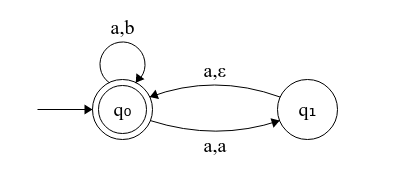
\includegraphics[scale=0.6]{mainmatter/images/e-d.png}
\caption{A-transducer $M'$}
\end{figure}

\paragraph{}
Clearly, $\C{M'} = 2$, $\C{A_{simple}} = 1$ and $\C{L_{p;adv}} = \floor{\frac{p}{2}} + 2$ (we look for the iteration of a string of length $\floor{\frac{p}{2}} + 2$ and one aditional state is for words with $b$ in incorrect positions). For $p \geq 11$, $\C{M'} + \C{A_{simple}} + \C{L_{p;adv}} \leq p$. \qed

\paragraph{}
\poznamka In the same way, we could prove the $T$-undecomposability of the languages $L_{p} = \{ (a^p)^+\}$,  where $p$ is a prime number (with Kleene plus instead of the star).

\paragraph{}
Similar result can be obtained for the class of $NT_{\forall}$-decomposable languages.

\paragraph{}
\cveta $\D{T} \subsetneq \D{NT_{\exists}}$

\paragraph{}
\dokaz The witness languages for this claim are the complements of $L_p$'s from previous Theorem. The $T$-undecomposability of $L_p^c$ can be proven in a very similar way than the $T$-undecomposability of $L_p$. We show just the first part of the proof, since the rest follows the same pattern as in aforementioned result.

\paragraph{}
Assume, that $L_{p}^c$ is $T$-decomposable. This means, that we can decompose $L_{p}^c$ into two languages $L_{p;trans}$ and $L_{p;simple}$, such that $L_{p;trans} \cap L_{p;simple} = L_{p}^c$. As we see, $L_{p}^c \subseteq L_{simple}$. However, since the finite automaton for $L_{p}^c$ has fewer than $p$ states, it is easy to see, that $L_{simple} \supseteq \{a^*\}$ (otherwise at least one of the words $a, aa, ..., a^{p-1}$ would be rejected). It  follows, that $L_{trans} \cap \{ a^k | k = 0 \pmod{p} \} = \emptyset$. As we  have said, the rest of the proof is almost identical to the proof of Theorem 20.

\paragraph{}
It remains to show, that for $p \geq 11$, $L_p^c$ is $NT_{\forall}$-decomposable. Once again, we use the a-transducer $M'$ from Figure 4.2 and this time, let $L'_{p;adv} = \{a,b\}^* \setminus (a^{\floor{\frac{p}{2}}}.b)^*$. We can find the language $M_{\forall}^{'-1}(L'_{p;adv})$ according to Lemma 16 as $M''(L'_{p;adv}) - M''(L_{p;adv}^{'c})$  for an a-transducer $M''$ dual to $M'$. It can be seen, that $M''(L'_{p;adv}) = \{a\}^*$ (in fact, to show this, it is sufficient to consider only the images of words from $b^*$). The language $M''(L_{p;adv}^{'c})$ was shown in the proof of previous Theorem - it is exactly $L_p$. Therefore, $M''(L'_{p;adv}) - M''(L_{p;adv}^{'c}) = \{a\}^* \setminus L_p$, which is exactly $L_p^c$. Moreover $L_{simple} = \{a\}^*$ and for $p \geq 11$, $\C{M'} + \C{L_{simple}} + \C{L_{p;adv}} = 2 + 1 + \floor{\frac{p}{2}} + 2 \leq p = \C{L_p}$ and it follows, that $L_p^c$ is $NT_{\forall}$-decomposable. \qed

\paragraph{}
\cveta $\D{NT_{\forall}} \subsetneq \R$, $\D{NT_{\exists}} \subsetneq \R$.

\paragraph{}
\dokaz The definition of $p$-decomposability for $p \in \{NT_{\exists},NT_{\exists}\}$ contains a requirement, that $L_{dec} = L[M_{p}^{-1}(L_{adv})](A')$ for some a-transducer $M$, regular language $L_{adv}$ and finite automaton $A'$. This condition can be rewritten as $L_{dec} = L(A') \cap M_{p}^{-1}(L_{adv})$. We have already seen, that $M_{p}^{-1}(L_{adv})$ can be found with an a-transducer $M'$ dual to $M$. It is well known, that the class of regular languages is closed under a-transduction, complement and intersection, so the claim, that $\D{NT_{\forall}} \subseteq \R$ and $\D{NT_{\exists}} \subseteq \R$ follows.

\paragraph{}
Moreover, the language $\{a\}^*$ is clearly regular, but since $\C{\{a\}^*} = 1$, we cannot decompose it into three models (a regular language, an a-transducer and a DFA), since each of them has at least one state. Therefore $\{a\}^* \notin \D{NT_{\forall}} \cup \D{NT_{\exists}}$. \qed

\paragraph{}
Previous theorem can be summarized in following hierarchy: \\

\centerline{$\D{A} \subsetneq \D{T}$ \stackanchor{\raisebox{-8px}{\begin{turn}{45}$\subsetneq $ \end{turn}} $\D{NT_{\forall}}$ \begin{turn}{315}$\subsetneq $\end{turn}}{\raisebox{10px}{\begin{turn}{315}$\subsetneq $ \end{turn}} $ \D{NT_{\exists}}$\begin{turn}{45}$\subsetneq $ \end{turn} }$ \R$}

\paragraph{}
As we have seen, the classes of regular languages concerning $T$-decomposability are different as the classes of A-decomposable and A-undecomposable languages. In the next part of our thesis, we investigate some properties of these classes.

%------------------------------------------------------------------------------------
\section{Closure properties}

\paragraph{}
When looking at a new class of languages, one of the first natural question, that arises, are its closure properties. In this section, we examine the closure of $T$-decomposable and $T$-undecomposable languages under some basic operations.

\subsection{$T$-undecomposable languages}
\paragraph{}
In this part, we mainly use two types of $T$-undecomposable languages. First of them are languages of type $L_p = \{ a^{pk} | k \geq 0 \}$ for $p$ a prime number. The $T$-undecomposability of these languages is proved in previous Section. The second type is the language $L = \{ a \}^*$. This language is clearly undecomposable, since $\C{L} = 1$ and all three devices contained in our foreign advisor concept have non-zero number of states.

\paragraph{}
\cveta The class of $T$-undecomposable languages is not closed under 
\begin{enumerate}
\item complement,
\item (non-erasing) homomorphism,
\item inverse homomorphism,
\item Kleene star, Kleene plus,
\item intersection,
\item union.
\end{enumerate}

\paragraph{}
\dokaz
\begin{enumerate}
\item \color{red}najst schodny dokaz, posledne dva nevysli\color{black}

\item Consider an undecomposable language $L_1 = \{ a^{13k} | k \geq 0 \}$ and a homomorphism $h:\{ a\}^* \to \{ a \}^*$, such that $h(a) = aa$. Clearly, $h(L_1) = \{ a^{26k} | k \geq 0 \}$ and this language can be decomposed in a following way: let us take a sequential transducer $M_1$ computing the identity mapping and a language $L'_1 = \{ a^{2k} | k \geq 0 \}$. This two items form the desired effective $T$-advice for $L_1$, since we only have for DFA $A$, such that $L(A) = \{ a^{13k} | k \geq 0 \}$, $L[M_{1,D}^{-1}(L'_1)](A) = L_1$.

Since this homomorphism is non-erasing, our class is not closed even under this kind of mapping.

\item \color{red}ToDo: najst nejaky schopny protipriklad\color{black}

\item \color{red}ToDo: dobra otazka, mozno nakoniec aj bude - ak ma jazyk  tvar $L^*$, potom asi musi byt v automate prechod akceptacny -> pociatocny a tu to vieme roztrhnut a potom ak sa dal zjednodusit ten cely, tak sa musi dat aj ten maly. lenze, tazko povedat, mozno sa ten jazyk tak nejak moze zvrhnut, ze sa to zrazu bude dat rozkladat. zistit!\color{black}

\item Consider two languages, $L_{41} = \{ a^{13k} | k \geq 1 \}$ and $L_{42} = \{ a^{2k} | k \geq 1 \}$. As stated before, both of these languages are $T$-undecomposable. However, $L_{41} \cap L_{42} = \{ a^{26k} | k \geq 1 \}$ is a $T$-decomposable language, as we have seen in the first part of this proof.

\item Let us take two languages, $L_{51} = \{ a^k | k \neq 0 \pmod{5} \}$ and $L_{52} = \{ a^k | k \neq 0 \pmod{7} \}$. The $T$-undecomposability of these languages was shown in Theorem 21.

\begin{figure}[h!]
\centering
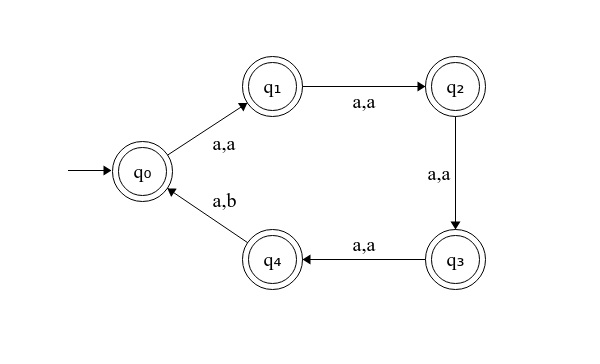
\includegraphics[scale=0.5]{mainmatter/images/M'_5.png}
\caption{Sequential transducer $M_5$}
\end{figure}

\paragraph{}
Now we claim, that the language $L_{53} = L_{51} \cup L_{52} = \{a^k|k\neq 0 \pmod{35}\}$ is $T$-decomposable. Clearly, $\C{L_{53}} = 35$. Take the sequential transducer $M_5$ from Figure 4.2. It can be seen, that the image of a word $a^{k}$ is a word from $\{a,b\}^*$ with the same length and if and only if $5 \mid k$, the last symbol of this output is $b$. Now, let $L_{adv} = \{a,b\}^* \setminus  (\{a,b\}^{7k-1}.\{b\})$. Clearly, $M_{5;D}^{-1}(L_{adv}) = L_{53}$. Then, $L_{simple} = \{a\}^*$ and clearly, $(L_{adv},M_5)$ is an effective $T$-advice with regard to $L_{53}$.

\end{enumerate} \qed

\subsection{$T$-decomposable languages}

\paragraph{}
\cveta The class of $T$-decomposable languages is not closed under 
\begin{enumerate}
\item complement,
\item (non-erasing) homomorphism,
\item inverse homomorphism,
\item Kleene star, Kleene plus,
\item intersection,
\item union.
\end{enumerate}

\paragraph{}
\dokaz
\begin{enumerate}
\item This claim follows directly from previous Theorem. \color{red}zatial previous theorem nie je\color{black}

\item Let us take a language $L_1 = \{w|w \in \{ a,b\}^* \wedge \#_{a}(w) \equiv 0 \pmod{42} \}$. Clearly, a language $L'_1 = \{w|w \in \{ a,b\}^* \wedge \#_{a}(w) \equiv 0 \pmod{14} \}$ with a sequential transducer $M_1$ computing the identity mapping is an effective advice for $L_1$.

Let us now consider a homomorphism $h: \{ a,b\}^* \to \{ a \}^*$, defined as $h(a) = a, h(b) = a$. Note, that $h$ is a non-erasing homomorphism. It easy to see, that $h(L_1) = \{ a \}^*$, however, as stated before, this language is $T$-undecomposable.

\item Consider a language $L_2 = \{ a^{26k} | k \geq 1 \}$. The decomposition of this language was shown in the proof of previous theorem. The desired homomorphism is $h: \{a\}^* \to \{a\}^*$, where $h(a) = aa$. Now, $h^{-1}(L_2) = \{ a^{13k} | k \geq 1 \}$, which is $T$-undecomposable.

\item The counterexample is a language $L_3 = \{ a^{11} \}$. Let us take a language $L'_3 = \{ a^{5} \}$; a sequential transducer $M_3 = (\{q_0, q_1, q_2\}, \{a\}, \{a\}, \delta, \sigma, q_0, \{q_1\})$, where\\
\centerline{$\delta(q_0,a) = q_1; \sigma(q_0,a) = \varepsilon$}
\centerline{$\delta(q_1,a) = q_2; \sigma(q_1,a) = \varepsilon$}
\centerline{$\delta(q_2,a) = q_1; \sigma(q_2,a) = a$}
and an automaton $A_3 = (\{q_0\}, \{a\}, \delta, q_0, \{q_0\}) $, where $\delta(q_0, a) = q_0$. Clearly, $M_{3;D}^{-1}(L'_3) = L_3$ and $\C{L'_3} + \C{T} + \C{A_3} = 5 + 3 + 1 \leq 9 = \C{L_3}$, therefore $L_3$ is $T$-decomposable. Though, $(L_3)^+ = \{ a^{11k} | k \geq 1 \}$ and $(L_3)^* = \{ a^{11k} | k \geq 0 \}$ are $T$-undecomposable.

\item Let us take a look at two languages, $L_{41} = \{ a \}^* \cup \{ b^{15k} | k \geq 1 \}$ and $L_{42} = \{ a\}^* \cup \{ c^{15k} | k \geq 1 \}$. We show the decomposition of $L_{41}$, since that of $L_{42}$ is very similar.

Let $L'_{41} = \{ a\}^* \cup \{ b^{3k} | k \geq 1 \}$ and $M_{41}$ compute the identity mapping. With this advice, we need to check just the language $L''_{41} = \{ a\}^* \cup \{ b^{5k} | k \geq 1 \}$ with an automaton $A''_{41}$. It is easy to see (and provable by Myhill-Nerode theorem), that a DFA for language $L_{41}$ needs at least $18$ states. However, $\C{L'_{41}} + \C{M} + \C{L''_{41}} = 6 + 1 + 8 = 15$ and clearly $L[L'_{41}](A''_{41}) = L_{41}$, which means, that $L_{41}$ is $T$-decomposable.

However, if we take the language $L_4 = L_{41} \cap L_{42} = \{ a\}^*$, we get a $T$-undecomposable language, therefore our class is not closed under intersection.

\item In previous section we have seen, that languages $L_{61} = \{a^{10}\}$ and $L_{62}=\{a^{12}\}$ are $T$-decomposable. Now we show, that also their complements are $T$-decomposable. Let $M_6 =(\{q_0,q_1,q_2\}, \{a\},\{a,b\},H,q_0,\{q_0,q_2\})$, where $H = \{(q_0,a,\varepsilon,q_1),\allowbreak (q_1,a,b,q_0),\allowbreak (q_0,a,a,q_2)\}$. It can be easily seen, that $M(a^{2k}) = b^k$ and $M(a^{2k+1}) = b^ka$. Now, the effective advice for $L_{61}^c$ consits of $M$ and $L_{61,adv} = \{b^5\}^c$. Clearly, $\C{M} + \C{L_{61,adv}} + \C{\{a\}^*} = 3+7+1 \leq 12 = \C{L_{61}^c}$ and $L_{61}^c = M^{-1}(L_{61,adv}) \cap \{a\}^*$. The effective advice for $L_{62}^c$ can be constructed in the same way.

However $L_{61}^c \cup L_{62}^c = \{a\}^*$ and since $\C{\{a\}^*} = 1$, this language is $T$-undecomposable.
\end{enumerate} \qed
